\documentclass[12pt]{article}
\usepackage{parskip, enumerate}
\usepackage{amsmath,pdfpages}
\usepackage{fancyvrb}
\usepackage[vlined,linesnumbered]{algorithm2e}
\usepackage[margin=.6in]{geometry}
\begin{document}
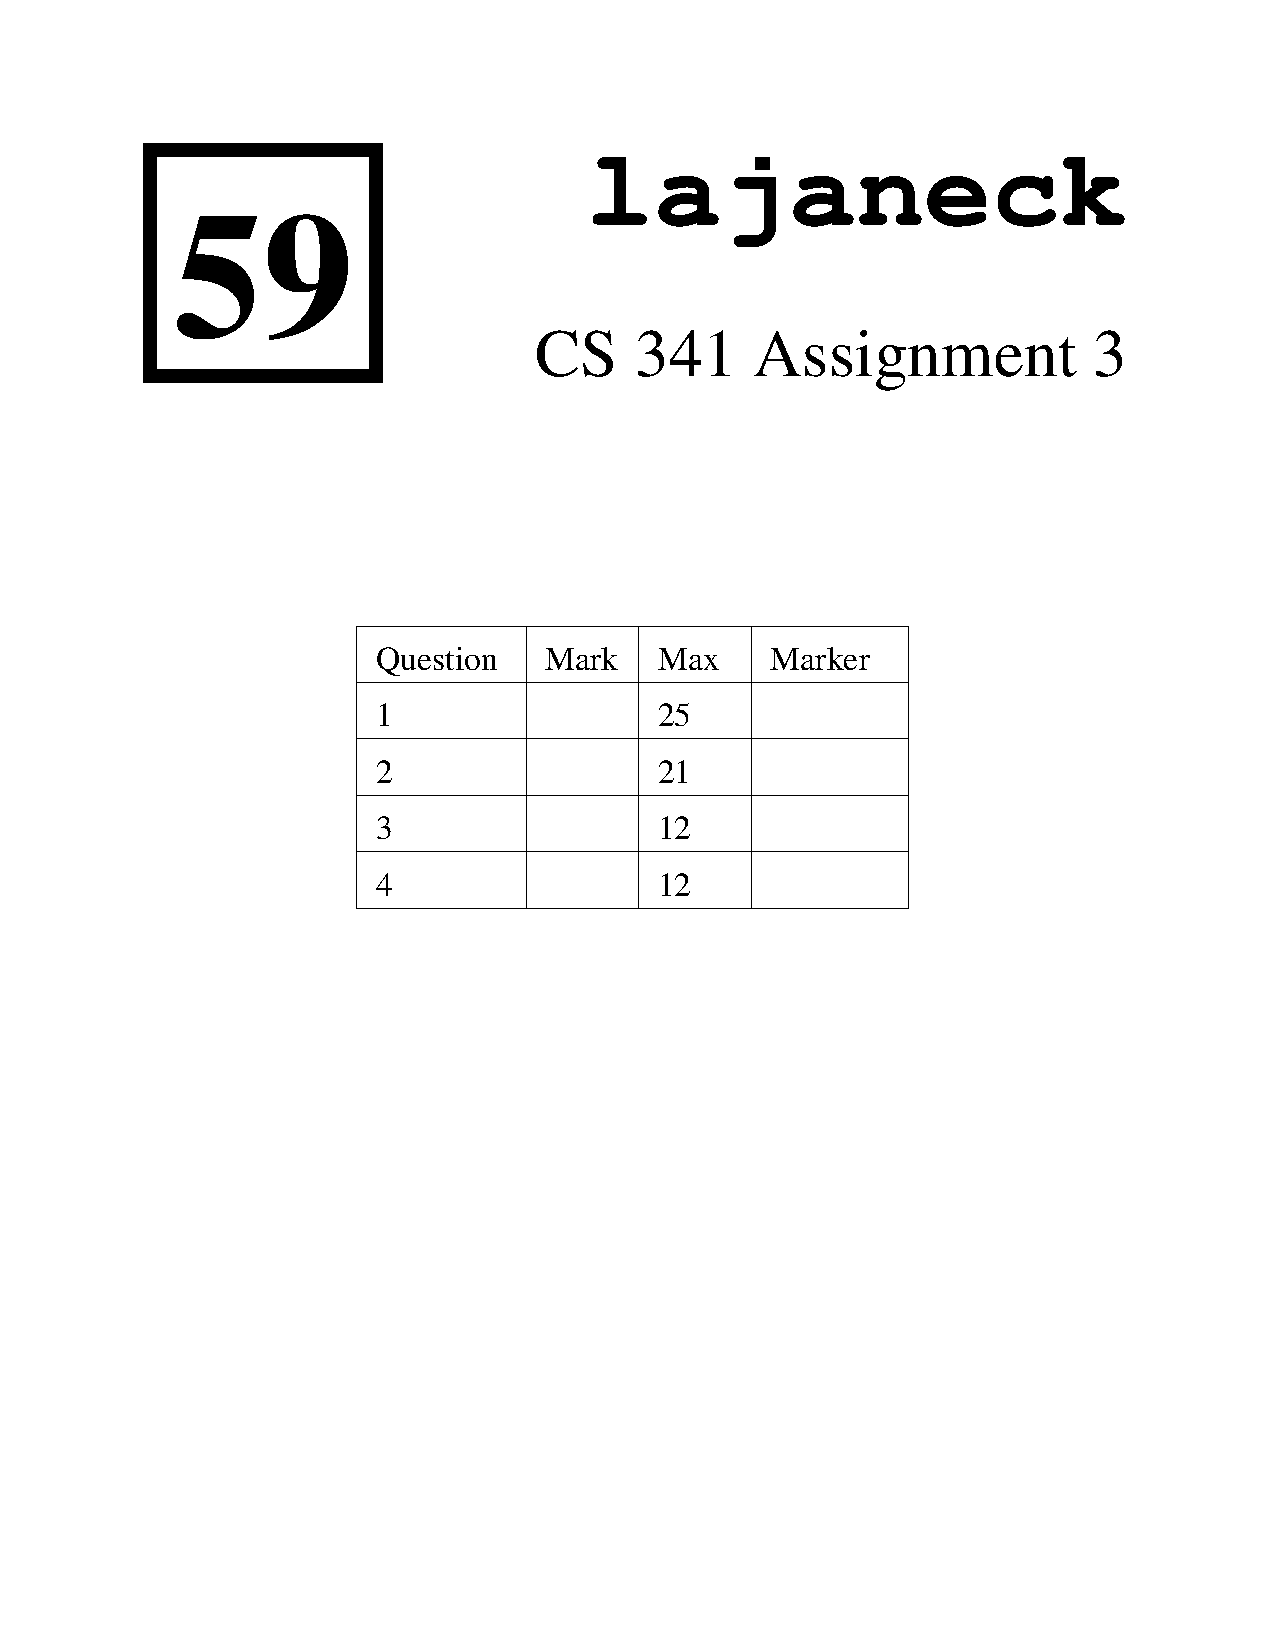
\includepdf[pages={1}]{cover.pdf}

\section*{Question 1}
\subsection*{a)}
\begin{eqnarray*}
    C[h,i,j] = \max \bigg( \displaystyle\sum_{k \in A} v_k + \displaystyle\sum_{l \in B} v_l  \bigg)\\
    \text { such that :} A \subseteq {1 \dots h} \text{,  }\\
    B \subseteq {1 \dots h},\\
    h \leq n, \\
    A \cap B = \phi, \\
    \displaystyle\sum_{k \in A} w_k \leq i \leq W, \\
    \displaystyle\sum_{l \in B} w_l \leq j \leq W
\end{eqnarray*}
A subproblem tries a h sized subset of the original n items, a max weight for backpack A of i, and a max weight for backpack B of j.

The answer for the original question is then $C[n,W,W]$.

\subsection*{b)}
If we have no items to pack we cannot pack any items so value must be 0, $C[0,i,j] = 0, \forall i,j$. Similarly if both A and B have maximum weights of 0 we cannot pack any items (since all items have positive non zero weights) and so have a value of 0, $C[h,0,0] = 0, \forall h$

\subsection*{c)}
When we include a new item, h, we have three choices: the item goes in A, B, or neither.

Case 1: The item goes in A. If by adding this item to A we make it weigh too much we cannot include it, so the value of A is the same as if we had not included h in our item subset, else the value increases by h's value. So:
\begin{center}
\[
 C_1 =
  \begin{cases}
   C[h-1, i - w_h, j]  + v_h & \text{if } i \geq w_h \\
   C[h-1, i, j]       & \text{else}
  \end{cases}
\]
\end{center}

Case 2: The item goes in backpack B. The same logic applies as in case 1.
\begin{center}
\[
 C_2 =
  \begin{cases}
   C[h-1, i, j - w_h]  + v_h & \text{if } j \geq w_h \\
   C[h-1, i, j]       & \text{else}
  \end{cases}
\]
\end{center}

Case 3: The item does not go in either backpack. Here we would have the exact same value as if we had not included h in the subset of items. So:
\begin{eqnarray*}
    C_3 = C[h -1,i,j]
\end{eqnarray*}

Of these three possible cases we want to achieve the maximum possible weight so we take the max of out choices.
\begin{eqnarray*}
    C[h,i,j] = \max(C_1, C_2, C_3)
\end{eqnarray*}

\subsection*{d)}
\begin{Verbatim}[numbers=left]
TwoKnapsackMaxSum(n, W){
    for(i = W downto 1) {
        for(j = W downto 1) {
            C[0,i,j] = 0
        }
    }
    for(h = n downto 1) {
        C[h,0,0] = 0
    }
    for(h = n downto 1){
        for(i = W downto 0){
            for(j = W downto 0){
                c1 = 0, c2 = 0, c3 = 0
                if(i >= w[h]}{ \\Case where the item is added to A
                    c1 = C[h-1, i-w[h], j] + v[h]
                }
                if(j >= w_h}{ \\Case where the item is added to B
                    c2 = C[h-1, i, j-w[h]] + v[h]
                }
                c3 = C[h-1,i,j] \\Case where the item is not added
                C[h,i,j] = max(c1, c2, c3)
            }
        }
    }
    return C[n,W,W]
}
\end{Verbatim}


\subsection*{e)}
To get the optimal subsets we maintain a second table D that keeps track of where the item went, A, B, or 0. Then we trace back from $C[n,W,W]$ applying the reverse formula based on what was done at that step to get where it came from.
\begin{Verbatim}[numbers=left]
TwoKnapsacOptimalSets(n, W) {
    for(i = W downto 1){
        for(j = W downto 1){
            C[0,i,j] = 0
            D[0,i,j] = 0
        }
    }
    for(h = n downto 1){
        C[h,0,0] = 0
        D[h,0,0] = 0
    }
    for(h = n downto 0){
        for(i = W downto 0){
            for{j = W downto 0) {
                c1 = 0, c2 = 0, c3 = 0
                if(i >= w[h]) {
                    c1 = C[h-1, i-w[h], j]  + v[h]
                }
                if{j >= w[h]}{
                    c2 = C[h-1, i, j-w[h]]  + v[h]
                }
                c3 = C[h-1,i,j]
                C[h,i,j] = max(c1, c2, c3)
                \\Updating D table with new item
                if(C[h,i,j] == c1){
                    D[h,i,j] = A
                }
                if(C[h,i,j] == c2){
                    D[h,i,j] = B
                }
                if(C[h,i,j] == c3){
                    D[h,i,j] = 0
                }
            }
        }
    }
    h = n
    i = W
    j = W
    while(h >= 0 && i >= 0 && j >= 0){
        if(C[h,i,j] = A){
            Add item h to set A
            h = h-1
            i = i-w[h]
        }
        if(C[h,i,j] = B){
            Add item h to set B
            h = h-1
            j = j-w[h]
        }
        if(C[h,i,j] = 0){
            h = h-1
        }
    }
    return (A,B)
}
\end{Verbatim}

\subsection*{f)}
TwoKnapsackMaxSum:\\
\begin{align*}
    \texttt{lines 2-6: } & \mathcal{O}(W^2) \text{ Since the body is constant time and is executed $W^2$ times}\\
    \texttt{lines 7-9: } & \mathcal{O}(n) \text{ Since the body is constant time and is executed n times}\\
    \texttt{lines 13-20: } & \mathcal{O}(1)\\
    \texttt{lines 10-25: } & \mathcal{O}(nW^2) \text{ Since the body is constant time and is executed $nW^2$ times}\\
    \texttt{total: } & \mathcal{O}(nW^2)
\end{align*}

TwoKnapsacOptimalSets:\\
\begin{align*}
    \texttt{lines 2-36: } & \mathcal{O}(nW^2) \text{ Since this is basically TwoKnapsackMaxSum with loop constant increased}\\
    \texttt{lines 41-53:  } & \mathcal{O}(1)\\
    \texttt{lines 40-54} & \mathcal{O}(n) \text{ Since h decreases by 1 each time and is bounded by n}\\
    \texttt{line 36: } & \mathcal{O}(1)\\
    \texttt{total: } & \mathcal{O}(nW^2)
\end{align*}

Space Usage:
Since each table is $n \times W \times W$ the space usage for TwoKnapsackMaxSum is nWW and TwoKnapsacOptimalSets is 2nWW (since it uses two tables);

\section*{Question 2}
\subsection*{a)}
C[i,j] = the minimum area for j non overlapping histogram rectangles containing points $P_1 \dots P_i$.

\subsection*{b)}
\begin{itemize}
    \item When we have no points we don't need any rectangles, so our area is 0, $C[0,j] = 0, \forall j$.
    \item If we have no rectangles, but at least one point there is no answer, so $C[i,0] = \infty, \forall i>0$.
    \item In any case where we have more rectangles than we have points we can get a area of 0 by giving each point its own 0 width rectangles, so $C[i,j] = 0, \forall i\leq j$.
\end{itemize}

\subsection*{c)}
Every time we add a new point we need to recalculate how we divide our boxes. We can do this by finding the optimal right most split. This means that for every point currently in our set we calculate the total area that would arise from taking that point and all points to its right as one box and dividing the rest of the points into j-1 boxes. By finding the minimum of these values we can find the optimal area for this new set of points.

\begin{eqnarray*}
    C[i, j] = \min(C[k-1, j-1] + Area(P_k \dots P_i)), \forall k \leq i
\end{eqnarray*}
$C[k-1, j-1]$ is the optimal area for all points left of k with j-1 boxes, and Area($P_k \dots P_i$) is the area of a rectangle required to contain all points from k to i. We then take the minimum of these to be the optimal area of this subproblem. This will give us the optimal answer because we will have tried every possible division of our set of points into boxes. The brute force way to do this is to make one block then check all other block combination of the remaining points, then repeat for every possible starting block size, but we already have the optimal division of leftover points in $C[k-1, j-1]$, so we only need to try every size of starting block and take the minimum.

\subsection*{d)}
\begin{Verbatim}[numbers=left]
MinHistogramArea(n, k){
    for{ j = k to 1 } {
        C[0,j] = 0
    }
    for(i = n downto 1 ){
        C[i,0] = infinity
    }
    for(j = k downto 1){
        for(i = n downto  0 ){
            if(j > i) {
                C[i,j] = 0
            }
            minArea = infinity
            maxY = 0
            for(k = i downto i ){
                if(P[k].y > maxY){
                    maxY = P[k].y //Updating the maximum y of the right most block
                }
                new = C[k-1, j-1] + (P[i].x-P[k].x)*maxY //Adding the area of the right most block to the optimal area of remaining points
                minArea = min(minArea, new)
            }
            C[i,j] = minArea
        }
    }
    return C[n, k]
}
\end{Verbatim}


\subsection*{e)}
To keep track of the block division for the optimal solution we need a secondary D table that hold the index of the pivot point, k that resulted in the minimum total area. From there we build a block of every point to the right of k and jump to the solution for the subproblem with k less points and 1 less block. Repeat this until there are no points left.

\begin{Verbatim}[numbers=left]
OptimalHistogramBlocks(n, k){
    for{ j = k to 1 } {
        C[0,j] = 0
        D[0,j] = 0
    }
    for(i = n downto 1 ){
        C[i,0] = infinity
        D[i,0] = infinity
    }

    for(j = k downto 1){
        for(i = n downto  0 ){
            if(j > i) {
                C[i,j] = 0
            }
            minArea = infinity
            maxY = 0
            pivot = i //The index of point that starts the right most block in the optimal solution
            for(k = i downto 1 ){
                if(P[k].y > maxY){
                    maxY = P[k].y
                }
                new = C[k-1, j-1] + (P[i].x-P[k].x)*maxY
                if(new < minArea){
                    minArea = new
                    pivot = k
                }
            }
            C[i,j] = minArea
            D[i,j] = pivot
        }
    }
    i = n, j = k, ret //Ret is a container of blocks in the optimal solution
    while(i > 0 && j > 0) {
        pivot = D[i,j]
        new = new Block containing P[pivot, ..., n] //Make new block of right most points past the pivot
        Add new to ret
        i -= pivot //Remove right most points from point set
        j -= 1 //Decrease number of blocks
    }
    return ret;
}
\end{Verbatim}

\subsection*{f)}
MinHistogramArea:\\
\begin{align*}
    \texttt{lines 2-4: } & \mathcal{O}(k)\\
    \texttt{lines 5-6: } & \mathcal{O}(n)\\
    \texttt{lines 9-14: } & \mathcal{O}(1)\\
    \texttt{lines 15-21: } & \mathcal{O}(i)\\
    \texttt{lines 9-23: } & \mathcal{O}(n^2) \text{ Sum from 1 to i of i is bounded by $n^2$}\\
    \texttt{lines 9-23: } & \mathcal{O}(n^2) \\
    \texttt{lines 8-24: } & \mathcal{O}(kn^2)\\
    \texttt{total: } & \mathcal{O}(kn^2)
\end{align*}

OptimalHistogramBlocks:\\
\begin{align*}
    \texttt{lines 2-32: } & \mathcal{O}(kn^2) \text{ This is the same as MinHistogramArea with adjusted constants}\\
    \texttt{lines 33-39: } & \mathcal{O}(kn)\\
    \texttt{total: } & \mathcal{O}(kn^2)
\end{align*}

\section*{Question 3}
We will divide the area into  $\mathcal{O}(n^2)$ rectangles by extending each line to infinity. Each rectangle will have a left, right, top, and bottom pointer. These pointers link each rectangle to rectangles that share a side with them. These rectangles are made by iterating through all lines from bottom up, left right. At each line intersection we make two new rectangles based on the direction we are moving (so as to not double count rectangles) and store these at that intersection. We then calculate the possible bounds and links for that rectangle. Previously created rectangles will have their upper bounds and links updated to correspond with these newly created rectangles. Then the next intersection can link its rectangles with previously made ones (provided there is not a real line fully separating them) and so on until we have a doubly linked (undirected) set of rectangles that we can traverse based on if you can legally move between them. From there we just need to find which rectangle s is in and run a DFS from there. If the rectangle containing t has been discovered we can say that we can travel from s to t.

Each rectangle must have access to its neighbors because we removed any neighbors that were separated by a solid line, so there can be no path from s to t that crosses a line. Every space in our area is also covered by us extending every line to infinity and building rectangles accordingly, so there can be no path from s to t that this solution does not cover.


\section*{Question 4}
Here we iterate through all disks, and for each disk we iterate through the remaining disks that intersect and attempt to assign them a color. If we reach a disk that has already been assigned a color different to the one we want to assign it then we have a situation where two disks of different colors overlap the same disk which means that the graph is not bipartite.


\begin{verbatim}
#include <iostream>
#include <vector>
#include <cmath>

struct disk {
    int x;
    int y;
    int r;
    int c; //color of 1 or 2
};

bool IsIntersecting(disk a, disk b) {
    return pow((a.x - b.x),2) + pow((a.y - b.y),2) <= pow((a.r + b.r),2);;
}

int flipColor(int c){
    if(c == 1){
        return 2;
    } else if(c == 2) {
        return 1;
    } else {
        return -1;
    }
}
int DiskColoring(std::vector<disk> A){
    std::string result = "";
    std::vector<disk>::iterator i = A.begin();
    std::vector<disk>::iterator j = A.begin();

    i->c = 1;
    for(; i != A.end(); i++){
        j = i;
        for(; j != A.end(); j++){
            if(i == j){
                continue;
            }
            if(IsIntersecting(*i, *j)) {
                if(j->c == i->c) {
                    std::cout << "0" <<std::endl;
                    return 0;
                } else {
                    j->c = flipColor(i->c);
                }
            }
        }
    }

    i = A.begin();
    for(; i != A.end(); i++){
        std::cout << i->c << " ";
    }
    std::cout << std::endl;

    return 1;
}

int main() {
    int n;
    std::vector<disk> A;

    std::cin >> n;
    for(; n > 0; n--){
        disk p;

        std::cin >> p.x;
        std::cin >> p.y;
        std::cin >> p.r;
        p.c = -1;

        A.push_back(p);
    }

    DiskColoring(A);
}
\end{verbatim}


\end{document}




